% vim: ts=2:sw=2:tw=80:et
\thispagestyle{fancy}
\pagestyle{fancy}

Configuration for device connections, clock definitions, signal routing, and
device paramters is performed using the \textbf{Configure Signals/Triggers, ...}
dialog.  This dialog can be opened by using the
\textit{Edit$\rightarrow$Configure Devices} menu item or by selecting the
\textit{wrench}/\textit{screwdriver} icon on the menu bar.  When Arbwave is
initially loaded, these actions create the dialog with empty configuration items
as shown in Fig.~\ref{fig:devcfg:empty}.

\begin{figure}[h!]
  \centerline{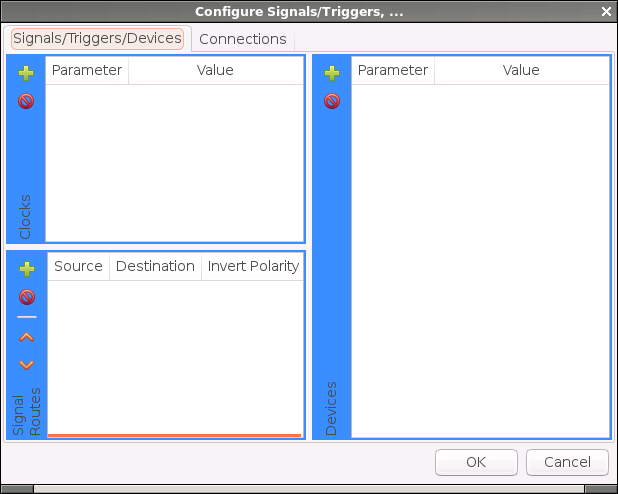
\includegraphics[width=.46\textwidth]{figures/empty}}
  \caption{Configuration window is empty upon startup}
  \label{fig:devcfg:empty}
\end{figure}


\section{Device Connections}\label{sec:devcfg:conn}
Typically, devices that are controlled by Arbwave would also be physically
connected to the same system on which Arbwave is running.  If this is the case,
the reader can skip this section and continue to Sec.\ref{sec:devcfg:clocks} to
configure the clocks.


\begin{figure}[h!]
  \centerline{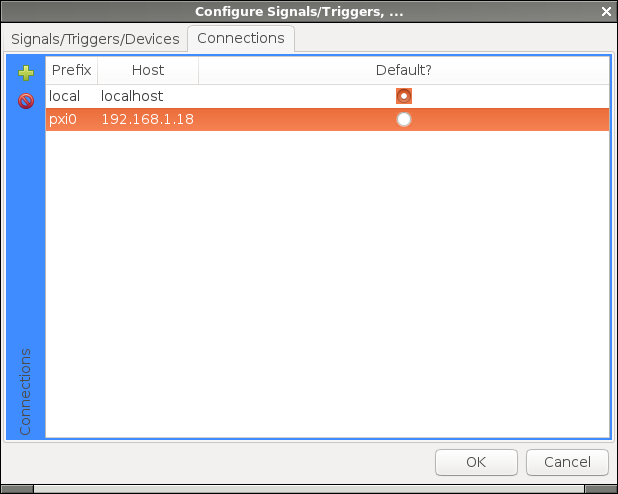
\includegraphics[width=.46\textwidth]{figures/connections}}
  \caption{Connection tab of configuration window with a default connection defined for
  the localhost and a non-default connection to a host with an alias defined as
  `pxi0'.}
  \label{fig:devcfg:connection}
\end{figure}

In addition to controlling devices that are physically connected to the local
machine, it is entirely possible to also control devices that are connected to
another machine that is running Arbwave in service mode (see
Sec.~\ref{sec:overview:cmdline} for relevant command line options).
These connections to remote devices are managed by the
\textbf{Configure$\rightarrow$Connections} tab, as shown in
Fig.~\ref{fig:devcfg:connection}.  On this tab, a user specifies an alias for a
connection as well as the host name for the connection.  For all connections,
nearly all paths will be prefixed by a
representation of the remote host or device.  For example, if a remote system is
identified by the word ``pxi0'', all paths from the corresponding devices of the
remote system will be prefixed by ``pxi0:''.  For example, `\texttt{ni/Dev1/ao0}' would become
`\texttt{pxi0:ni/Dev1/ao0}'.  A user can also specify a default host.  In this case, any
path that does not have the proper ``host:'' prefix will be interpreted to mean
the default connection.

The default configuration for connections are
\begin{lstlisting}
(prefix='local', host='localhost', default=True)
\end{lstlisting}


\section{Clocks}\label{sec:devcfg:clocks}

\subsection{General Discussion}
Analog and digital output cards generally have the notion of changing the output
levels at times based upon some digital clock pulse.  In general, there are two
strategies implemented by device manufacturers for generating output
samples/updates:

\begin{itemize}
\item \textbf{Update/Sample per Clock}\\
  A very typical timing implementation of data acquisition hardware is to cause
  an update (change in output) for each time that a clocks pulse is received by
  the hardware.  For example, a particular hardware device will have a list of
  output values that it is to generate.  Each time that the rising edge
  (usually) of a clock pulse is detected, the circuitry of the particular
  hardware device reads the next output value and sets its actual output
  accordingly.  A side effect of this strategy is to easily overburden device
  memory or device communication bandwidth.  This is because the data must be
  padded throughout an output waveform if ever any clock pulse is desired to not
  change the output.  This very often occurs if either a fixed update clock is
  used or if more than one hardware device is connected to the same clock.

  In spite of the high potential to waste device/system resources, Arbwave does
  simplify the use of this type of hardware.  For hardware devices configured to
  operate with this type of update clock, the output data will automatically be
  padded with the timing of each update/sample (padded or real) calculated to
  the nearest clock pulse.

\item \textbf{Programmed Update/Sample Output}\\
  Some hardware limits the waste of device resources by using an associated
  timestamp for each update/sample.  By comparing the given timestamp to a count
  of the device's clock source, an arbitrary delay can be accomplished between
  updates/samples.  Arbwave automatically calculates the timestamps to the
  nearest transition of the device's clocks source.
\end{itemize}

\subsection{Digital Channels as Clocks}
Because of the automatic coordination performed by Arbwave, it is possible to
use these two update types in concert in order to maximize the device resource
savings.  Most digital output backend components in Arbwave provide for digital
output channels to be used as timing/clock sources for other devices.
For example, a typical Arbwave configuration uses at least one channel
of \textbf{Programmed Update/Sample Output} digital hardware (e.g. Viewpoint
DIO-64, Marvin Test GxFpga with \acro{AFRL} firmware, or \acro{AFRL} Timing Cape
for Beaglebone Black) to generate the clock pulses of
\textbf{Update/Sample per Clock} hardware (e.g most \acro{DAQmx}, \acro{COMEDI}
hardware).  It is important to note that digital channels configured as clocks
\textit{cannot} also be configured as normal output channels.

For this type of configuration, the clock rate will automatically change such
that the minimum number of clocks are emitted to support all channels/devices
tied to the clock.  Clock pulses are designed to allow all voltage transitions
as specified at their transition time within the maximum clock resolution
possible (the internal clock rate of the DIO-64 for example).  In other words, a
single waveform element may have a variable clock depending on whether other
waveform channels similarly clocked need to have transitions in the mean time.


\subsection{Clock Assignment}
In order for Arbwave to correctly coordinate and visualize the multitude of
digital/analog transitions, each output device must have a driving clock
assigned to it explicitly.  In other words, all devices, regardless whether they
use an external clock source or an internal clock to define time, must have a
clock clock assignment in Arbwave.  These assignments allow Arbwave to correctly
coordinate and visualize each output transition.  As discussed in
Secs.~\ref{sec:devcfg:clkdef}-\ref{sec:devcfg:devices}, Clock assignment is
performed by
%
\begin{enumerate}
  \item defining clock sources (Sec.~\ref{sec:devcfg:clkdef})
  \item defining signal sources (Sec.~\ref{sec:devcfg:routes})
  \item configuring device clock sources (Sec.~\ref{sec:devcfg:devices})
\end{enumerate}


\section{Clock Definitions}\label{sec:devcfg:clkdef}
\begin{figure}[ht!]
  \centerline{
    a) 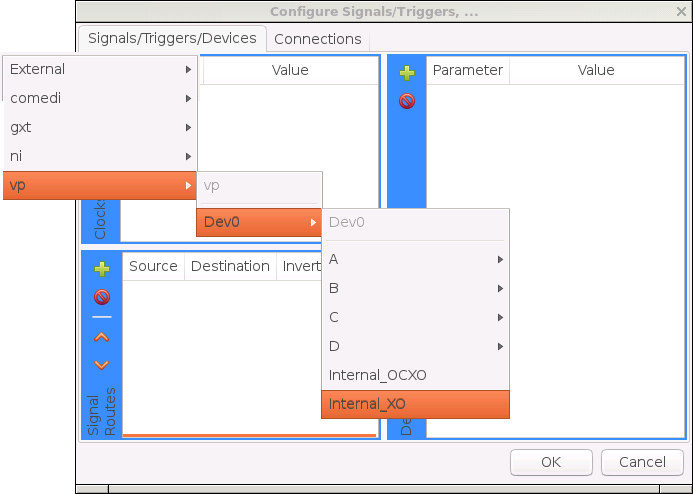
\includegraphics[width=.46\textwidth]{figures/add-clock-vp-XO}
    \hspace{.2em}
    b) 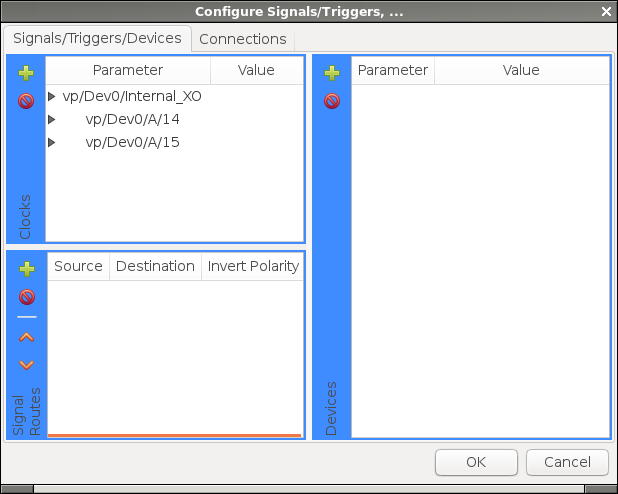
\includegraphics[width=.46\textwidth]{figures/clocks-added}
  }
  \caption{
    a) Viewpoint DIO-64 internal crystal oscillator configured as clock source.
    b) Two DIO-64 channels also configured as clock sources.
  }
  \label{fig:devcfg:clocks-added}
\end{figure}
%
%
Each clock must first be defined in the \textit{Clocks} section of the
\textbf{Configure$\rightarrow$Signals/Triggers/Devices} tab.
Fig.\ref{fig:devcfg:clocks-added}a shows an example of telling Arbwave about the
internal timing source provided by a Viewpoint DIO-64 card.
Fig.\ref{fig:devcfg:clocks-added}b shows two digital output channels of the
DIO-64 card configured as clock sources to be used by other devices.



\section{Signal Routes}\label{sec:devcfg:routes}
Signal routes are connections of various signals (triggers, clocks, \ldots)
within an experimental setup.  Many manufacturers provide the means to
connect these various signals to a device for use as trigger or clock signals.  By
using the \textit{Signal Routes} section of the
\textbf{Configure$\rightarrow$Signals/Triggers/Devices} tab, the user provides
information to Arbwave about which signals are either externally connected or
require to be connected using internal multiplexers built into the
various device hardware.

For example, consider the clock configuration example begun in
Sec.~\ref{sec:devcfg:clkdef}.  If we want to use the digital output channels
\signal{vp/Dev0/A/14} and \signal{vp/Dev0/A/15} as possible clock sources for
another device, such as \device{ni/Dev1/ao}, it is necessary to define how these
digital channels are routed to the \signal{ao/SampleClock} input signal of the
\device{ni/Dev1/ao} device.  For this particular hardware, two signal paths are
possible:
\begin{enumerate}
  \item A external connection using a physical cable.  In this case, we give the
    particular cable a name to define a signal route such as
    \signal{vp/Dev0/A/14} $\rightarrow$ \signal{External/cable0} $\rightarrow$
    \signal{TRIG/x}.  The first two lines of the \textit{Signal Routes} section
    shown in Fig.~\ref{fig:devcfg:routes-added} demonstrate this signal route
    defined for Arbwave.
  \item A direct signal route through the backplane (or \acro{RTSI} for PCI
    devices) signal bus.  Such a route could be represented as
    \signal{vp/Dev0/A/15} $\rightarrow$ \signal{TRIG/x}.  The last line of the
    \textit{Signal Routes} section shown in Fig.~\ref{fig:devcfg:routes-added}
    demonstrate this signal route defined defined for Arbwave.
\end{enumerate}


\begin{figure}[ht]
  \centerline{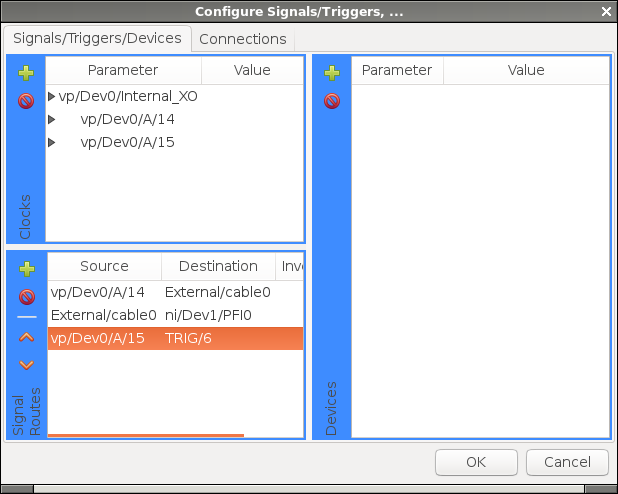
\includegraphics[width=.46\textwidth]{figures/routes-added}}
  \caption[Signal routes configuration]{
    Configuration window after defining signal routes for digital channels used
    as clocks.
  }
  \label{fig:devcfg:routes-added}
\end{figure}


\section{Devices Configuration}\label{sec:devcfg:devices}
Various configuration parameters for individual devices can be set using the
\textit{Devices} section of the
\textbf{Configure~$\rightarrow$~Signals/Triggers/Devices} tab.  Continuing our
configuration example, we use add the \device{vp/Dev0} and \device{ni/Dev1/ao}
devices to the \textit{Devices} section.  For each of these devices, various
configurable options appear.  Using the interface shown in
Fig.~\ref{fig:devcfg:devices}, it is possible to configure trigger options,
buffer options, and so forth.

\begin{figure}[htb!]
  \centerline{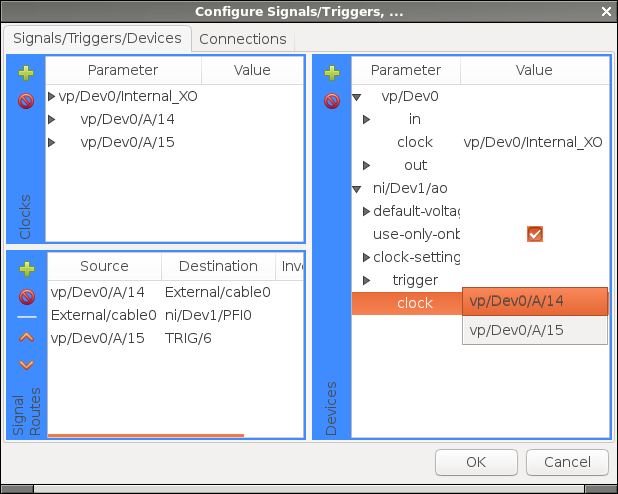
\includegraphics[width=.46\textwidth]{figures/devices-set-clocks}}
  \caption{Configuration window after assigning appropriate clocks to
  devices}
  \label{fig:devcfg:devices}
\end{figure}

\subsection{Clock Sources for Devices}\label{sec:devcfg:clksrc}
Each device configured in the \textit{Devices} section will also have a
\textbf{clock} configuration item.  As indicated earlier, this clock-source
configuration item is mandatory for every device used by Arbwave.  It should be
noted that Arbwave only allows clocks in the \textit{Clocks} section to be
selected as device-clock sources.  This means that each clock and its associated
signal routing must first be configured in order to be used as a clock source.

Continuing our example, we have defined two possible clock sources
(\signal{vp/Dev0/A/14} and \signal{vp/Dev0/A/15}) and their associated signal
routes.  Internally, a \device{ni/Dev1/ao} analog device has the ability to use,
among several other possibilities, an external BNC connection or even a
backplane (PXI or \acro{RTSI}) bus connection to receive a update/sample clock
pulse (denoted \signal{ao/SampleClock}).  Arbwave uses the \textit{Clocks} and
\textit{Signal Routes} information to allow the user to select the actual clock
source, as shown in the pop-up menu in Fig.~\ref{fig:devcfg:devices}.
